\documentclass{standalone}

\usepackage{amssymb}
\usepackage{amsthm}
\usepackage{amsmath}


\usepackage{tikz}
%\usetikzlibrary{shapes,backgrounds,calc,patterns}
%\usepackage{venndiagram}


\begin{document}

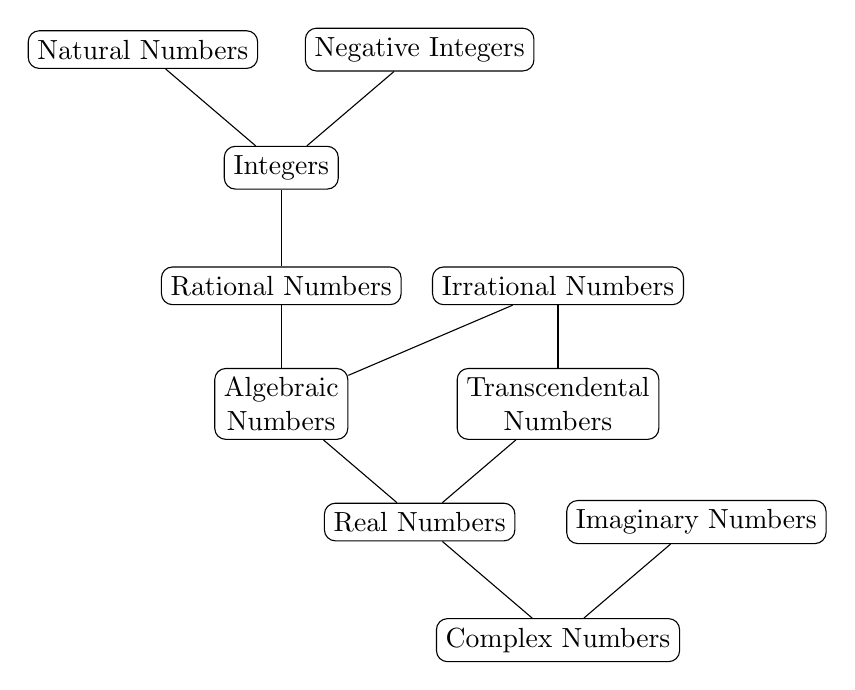
\begin{tikzpicture}[sibling distance=10em,
every node/.style = {shape=rectangle, rounded corners,
	draw, align=center}]]
	\node {Complex Numbers}[grow=up]
		child {node {Imaginary Numbers}}
		child {node {Real Numbers}
			child {node {Transcendental \\ Numbers}
				child {node(Irrational) {Irrational Numbers}}}
			child {node(Algebraic) {Algebraic \\ Numbers}
				child {node {Rational Numbers}
					child {node {Integers}
						child {node {Negative Integers}}
						child {node {Natural Numbers}}}}}};
	\draw (Algebraic) -- (Irrational);
\end{tikzpicture}
\end{document}